\chapter{Related Works}

\section{Learning Discrete CA with Genetic Algorithms}

\noindent
\textbf{Learning Algorithm for Modeling Complex Spatial Dynamics} (Meyer, Richards, and Packard, 1989) \cite{meyer1989learning} is a seminal work in this area. It creates a dynamical model from observations of discrete values evolving on a lattice over time. The model is represented as a binary probabilistic cellular automaton (PCA) whose neighbourhood set is learned by a genetic algorithm. The motivation for this work is to establish the form of CA which would most accurately describe patterns in the physical world directly from experimental data of physical interactions. In particular, Richards et al. \cite{richards1990extracting} builds on these techniques to find PCA rules that accurately predict the evolving patterns generated by the dendritic solidification of NH\textsubscript{4}BR.\\

Note that this goal is different from learning the entire transition function of a cellular automaton. This work merely aims to establish \textit{which} parameters in a local vicinity of the current state are most relevant to predicting the future state, not \textit{how} those parameters are combined and transformed to produce the future state.\\

The aim is to discover the most appropriate local neighbourhood set within a vicinity from the central cell that extends two steps in both space and time. This is the intersection of the Moore neighbourhood in time step $t-1$ and the von Neumann neighbourhood of range 2 in time step $t-2$. This comes to a 20 cell neighbourhood in space and time as visualised in Figure~\ref{fig:20-near}.

\begin{figure}[!h]
\centering
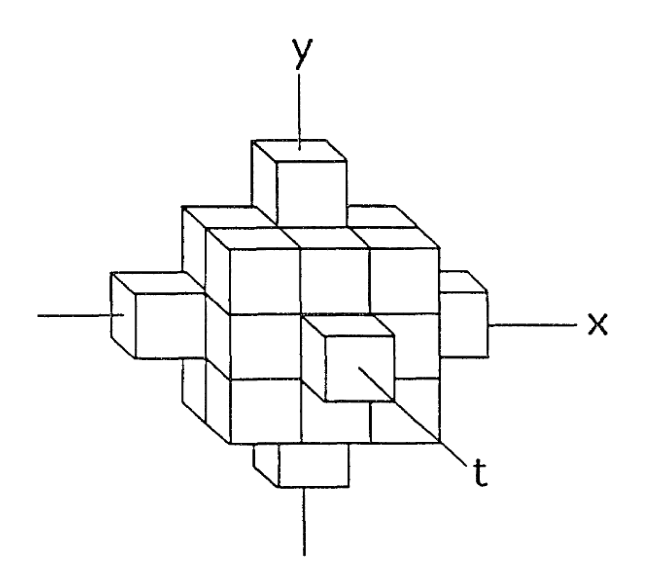
\includegraphics[width=0.3\textwidth]{images/20_neighbourhood.png}
\caption{20-cell, two step neighbourhood in space and time}
\label{fig:20-near}
\end{figure}

The full 20-cell neighbourhood is called the master template and each chromosome encodes some subtemplate ${s_1, ..., s_m}$. The fitness function used is
\begin{align*}
                    F &= I - \frac{2^m}{N}\\
    \text{where\:}  I &= \sum P(s, s_1,, ..., s_m)\log_2{\frac{P(s, s_1, ..., s_m)}{P(s)P(s_1, ..., s_m)}}
\end{align*}
Here, $I$ is the mutual information of the subtemplate and represents the amount of information (measured in Shannon bits) about the value of the central cell that can be obtained from the states of the cells in the subtemplate. It is calculated by summing across all $2^m$ configurations of the subtemplate in the data and across both values of $s \in \{0,1\}$. The second term in the fitness function ensures that subtemplates of varying sizes are treated appropriately by proportionately penalising large subtemplates that, by nature, will contain more information. In our case, $N=20$\\

The genetic algorithm initialises the population randomly. At each time step, a linear ranking of candidiates is performed and truncation selection is performed to pick the fittest subset. Crossover is applied between pairs of randomly selected candidates where the crossover point is an arbitrary cut in space-time on the master template. Point mutation is applied by either adding or removing a single cell from each candidate. This process is iterated to converge towards an optimum.\\

This method was successful at learning test data generated from a 1 time step Moore neighbourhood and data generated from 1 time step von Neumann neighbourhood with range 2. The algorithm successfully reproduces patterns generated by the first dataset precisely. However, unlike the first goal, the second goal neighbourhood is not subsumed by the master template. This means the algorithm can only hope to learn a similar template, not the exact objective. Despite this, the algorithm was able to find a neighbourhood set that produced correct behaviour 96\% of the time.\\

As the first notable exploration of learning CA properties with genetic algorithms, this paper devised a novel method for learning neighbourhood sets on binary PCA. It demonstrates the ability of this algorithm to predict neighbourhoods interior to the allocated search space as well as close approximations for objectives outside the search space.\\

This work raised many questions for future research. The most pertinent is whether it is possible to link learned rules to existing and future theoretical models. This work also only explored binary state CA but this excludes many continous variables relevant to data obtained from physical reactions such as the temperature field. An exploration of similar techniques on continous-state CA could be explored to closer approximate the partial differential equations that underlie the processes being explored.\\

Finally, this paper focused only on identifying the neighbourhood set of the CA that would closely approximate the interactions being studied. For the purposes of this thesis, we are interested in going beyond this and approximating the full transition function. In some cases we will fix the neighbourhood function used to reduce our search space under the assumption that further research could use techniques outlined in this paper to test whether better sub-neighbourhoods exist.